\documentclass[aspectratio=169]{beamer}

\usepackage[T1]{fontenc}
\usepackage[utf8]{inputenc}
\usepackage[english]{babel}
\usepackage{pgfplots}
\pgfplotsset{compat=newest}
\usepackage{booktabs}
\usepackage{siunitx}

\usepackage{tikz}

\usefonttheme{professionalfonts}
\usepackage{fontspec}
\setsansfont
  [Ligatures=TeX, % recommended
   UprightFont={* Light},
   ItalicFont={* Light Italic},
   BoldFont={* Medium},
   BoldItalicFont={* Medium Italic}]
  {Neo Sans Std}
%\setromanfont{Neo Sans Std}

% Remove Figure word from caption
\setbeamertemplate{caption}{\raggedright\insertcaption\par}


\usepackage{mathtools}

\usepackage{unicode-math}
\setmathfont{TeX Gyre Pagella Math}

% Latin Modern
%\usepackage{lmodern}
% Verdana font type
%\usepackage{verdana}
% Helvetica
%\usepackage{helvet}
% Times (text and math)
%\usepackage{newtx, newtxmath}

\usetheme[department=elektro,showsection=true]{DTU}

\setbeamertemplate{section page}
{
\color{white} {\large \insertsection}
%\par
}

\AtBeginSection[]{
\begingroup
\setbeamercolor{background canvas}{bg=dtured}
\frame[dtuwhitelogo,noframenumbering]{\sectionpage}
\endgroup
}

\title[PhD defence]{Demand Response for a Secure Power System Operation}
\subtitle{Service Specification, Validation and Verification in view of Distributed Energy Systems}
\author{Daniel Esteban Morales Bondy}
\institute{Energy Systems Operation and Management\\ Center for Electric Power and Energy \\ Technical University of Denmark \\ \vspace{1cm} \today}
\date{\today}
	
\newcommand{\tabitem}{{\color{dtured}$\bullet$} }

\begin{document}
\frame{
	\maketitle
}

\frame{
	\frametitle{Outline}
	\tableofcontents
}

\section{Introduction}
\subsection{Changes in the power system}
\frame{
	\frametitle{Energy supply must be sustainable and clean}
	The world faces:
	\begin{itemize}
	\item[] Climate issues
	\item[] Health issues
	\item[] Geopolitical issues
	\end{itemize}
	\vspace{1cm}
	The Danish solution: 
	\begin{itemize}
	\item[]50\% of electricity generated by wind in 2020
	\item[]Full coverage of electricity and heat supply by renewable energy in 2035
	\item[]Fossil fuel independent by 2050
	\end{itemize}
}

\frame{
\frametitle{From production follows consumption to \\ consumption (partly) follows production}
\setbeamercovered{transparent}
\begin{figure}
	\begin{minipage}[b]{0.3\linewidth}
	\centering
	\includegraphics<1>[width=\textwidth]{figures/traditional_grid_new.eps}
	\includegraphics<2->[width=\textwidth]{figures/traditional_grid_new_tr.eps}
	\caption{\uncover<1>{The traditional power system, where energy flows from producer to consumer.}}
	\end{minipage}
	\hspace{3cm}
	\begin{minipage}[b]{0.3\linewidth}
	\centering
	\includegraphics<1>[width=\textwidth]{figures/smart_grid_new_tr.eps}
	\includegraphics<2->[width=\textwidth]{figures/smart_grid_new.eps}
	\caption{\uncover<2->{The future power system includes renewable generation and advanced ICT.}}
	\end{minipage}
\end{figure}
%\begin{figure}
%
%
%\end{figure}
%
%\begin{figure}
% \hspace{2cm}
%\includegraphics[width=0.3\columnwidth]{figures/}
%\caption{}
%\end{figure}
}

\frame{
\frametitle{The Demand Response Aggregator \\ is a new service provider}
\begin{figure}
\centering
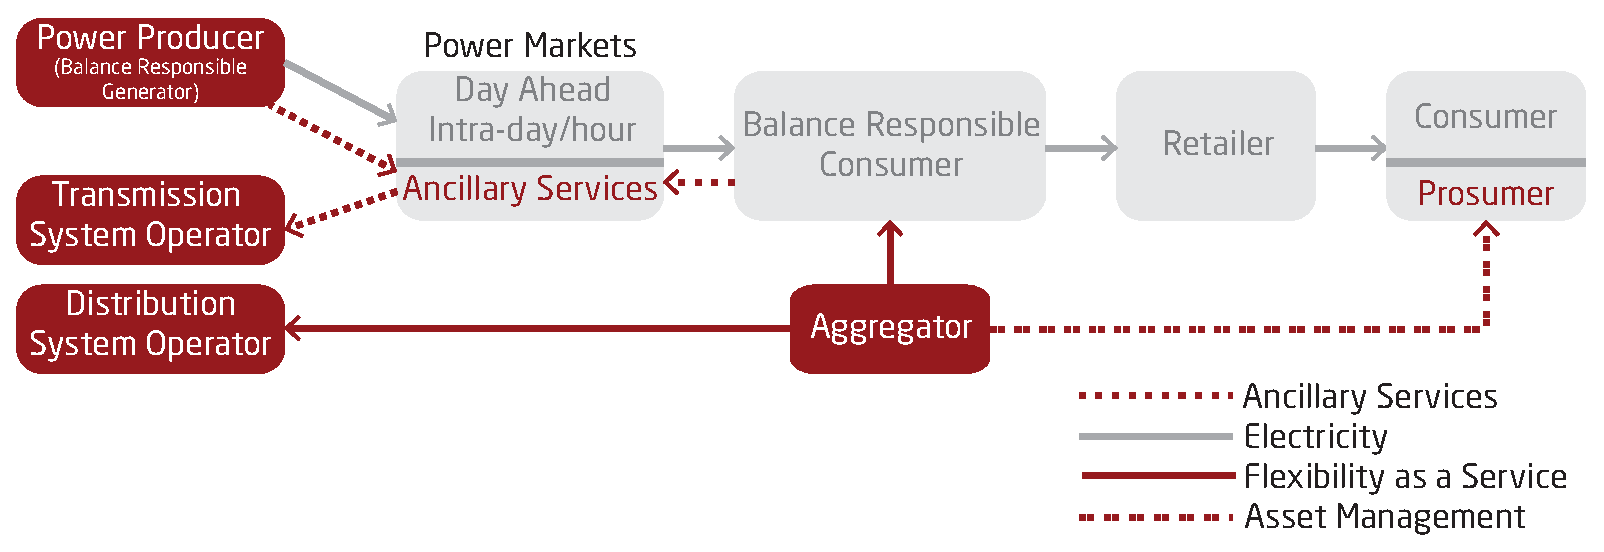
\includegraphics[width = 0.7\textwidth]{figures/market_future.eps}
\caption{A future market setup with an independent aggregator.}
\end{figure}
}

\frame{
\frametitle{How do we ensure aggregator reliability?}
\begin{itemize}
\item[1.-] How do we validate aggregators?
\item[2.-] Which are the service needs aggregators satisfy?
\item[3.-] How do we quantify performance in service delivery?
\end{itemize}
}




\section{The Aggregator}
\frame{
\frametitle{A reference architecture is needed in order to\\ have a common understanding of what an aggregator is}
\begin{columns}[c,onlytextwidth]
	\begin{column}{.5\textwidth}
	\setlength{\partopsep}{0pt}
		A reference architecture must provide:
			\begin{itemize}
			\item[] A common lexicon and taxonomy
			\item[] Modularization and complementary context
			\item[] A common architectural vision
		\end{itemize}
	\end{column}
	
	\begin{column}{.5\textwidth}
		\begin{center}
		\begin{figure}
		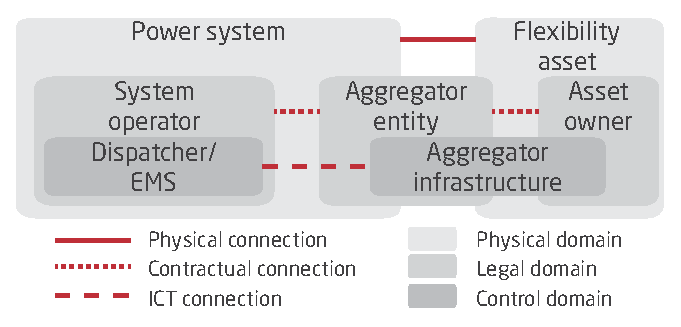
\includegraphics[width=\columnwidth]{figures/domains3.eps}
		\caption{The aggregator concept spreads across domains.}
		\end{figure}
		\end{center}
	\end{column}
\end{columns}
}
\frame{
\frametitle{AggrefArch}
		\begin{center}
		\begin{figure}
		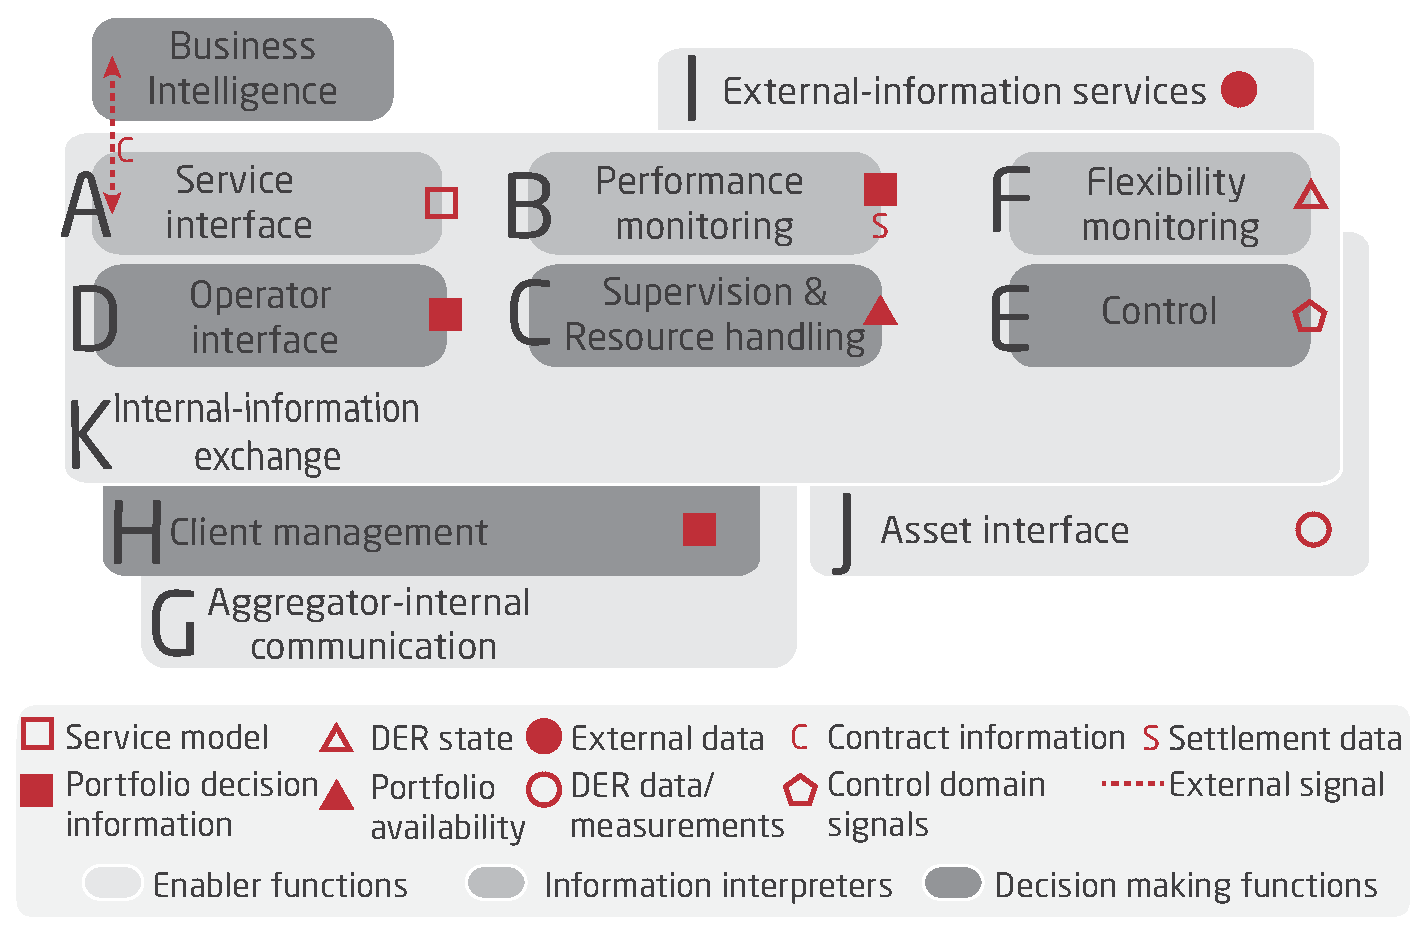
\includegraphics[width=.6\textwidth]{figures/diag_simple3.eps}
		\caption{The aggregator functional reference architecture abstracts from specific control architectures.}
		\end{figure}
		\end{center}
}

\frame{
\frametitle{Relevance of the reference architecture}
Contributions/conclusions are listed here
}

\section{How do we validate aggregators?}

\frame{
\frametitle{Aggregators are essentialy different from generators}
\begin{columns}[c,onlytextwidth]
	\begin{column}{.5\textwidth}
	\setlength{\partopsep}{0pt}
		\begin{itemize}
			\item[] Heterogeneous in composition: can not be described by a single equation
			\item[] Geograghically distributed: no single point of measurement
			\item[] Different failure modes: reliability must be evaluated differently
			\item[] Architectures vary: new operating conditions are relevant
		\end{itemize}
	\end{column}
	
	\begin{column}{.5\textwidth}
		\begin{center}
			\begin{figure}
			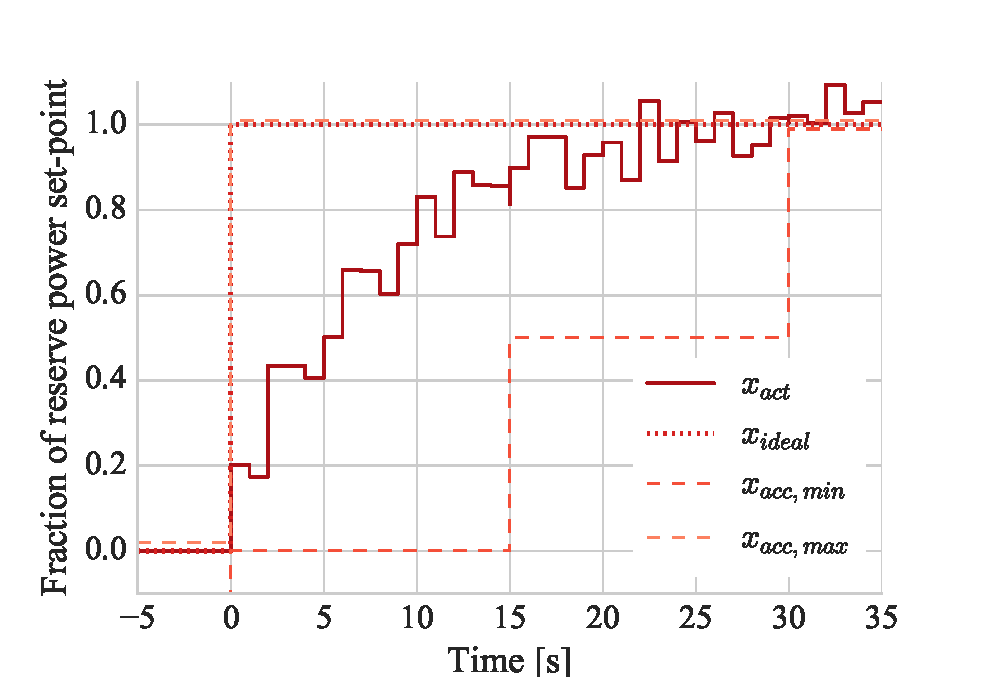
\includegraphics[width=0.8\textwidth]{figures/primfreqresp2.eps}
			\caption{Example of an aggregator response to step input.}
			\end{figure}
		\end{center}
	\end{column}
\end{columns}
}

\frame{
\frametitle{Current procedures are insufficient due to the \\ differences between aggregators and generators}
%\setbeamercovered{transparent}
\begin{columns}[c,onlytextwidth]
	\begin{column}{.5\textwidth}
	\setlength{\partopsep}{0pt}
		\only<1>{Current procedure:}
		\only<2->{New procedure:}
		\only<1>{
		\begin{itemize}
			\item[] Documentation
			\item[] Prequalification test
		\end{itemize}
		}
		\only<2->{
		\begin{itemize}
			\item[] Documentation
			\item[] Simulation test
			\item[] Prequalification test \& Monitoring
		\end{itemize}
		}
	\end{column}
	
	\begin{column}{.5\textwidth}
		\begin{center}
			\begin{figure}
			\includegraphics[width=\textwidth]{figures/swissresponse.eps}
			\caption{Prequalification signal in SwissGrid}
			\end{figure}
		\end{center}
	\end{column}
\end{columns}
}

\frame{
\frametitle{Validation of aggregators must rely on \\ statistical Design of Experiments}
\begin{columns}[c,onlytextwidth]
	\begin{column}{.5\textwidth}
	\setlength{\partopsep}{0pt}
		New procedure:
		\begin{itemize}
			\item[] Documentation
			\item[] Prequalification test
		\end{itemize}
		
	\end{column}
	
	\begin{column}{.5\textwidth}
		\begin{center}
			\begin{figure}
			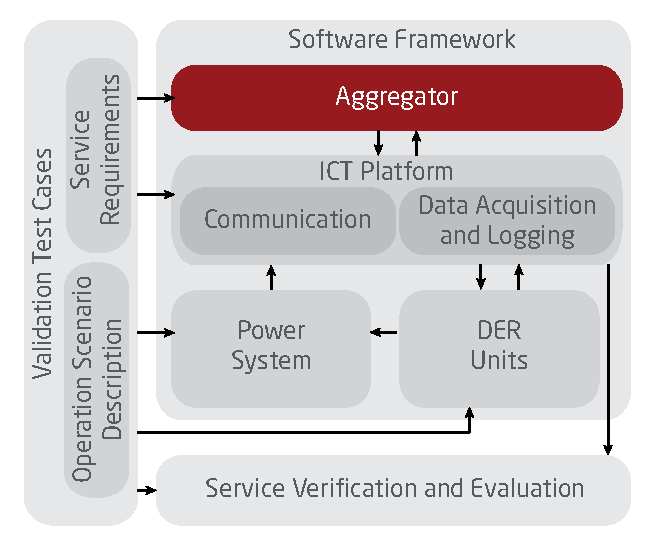
\includegraphics[width=0.7\textwidth]{figures/framework.eps}
			\caption{Conceptual validation framework}
			\end{figure}
		\end{center}
	\end{column}
\end{columns}
}


{\setbeamercolor{background canvas}{bg=black}
\frame[dtuwhitelogo]{some text}}
\section{Which are the service needs aggregators satisfy?}

\section{How do we quantify performance in service delivery?}


%{
%\setbeamercolor{background canvas}{bg=black} % Background color
%	\frame[dtuwhitelogo]{
%		\frametitle{Hello Blackness}
%		Here is another frame style!
%	}
%}

\section{Conclusion}


%================================================
%===  Define the contact details
\newcommand\contactTable{ %
  \begin{tabular}{lr}
    \multicolumn{2}{l}{Daniel Esteban Morales Bondy} \\ 
    \multicolumn{2}{l}{CEE, Technical University of Denmark (DTU)} \\ \midrule
    Building 776, Room 119    & bondy@elektro.dtu.dk. \\
    4000 Roskilde, Denmark & +45 30139930
  \end{tabular}
}%

\frame[dtuwhitelogo, bgfilename=dtu_bg_fiber]{ % 
  \begin{tikzpicture}[remember picture,overlay]
    \node[fill=black, fill opacity=0.9, 
          text=white, text opacity=1.0,
          rounded corners=5pt, 
          font=\scriptsize] at (current page.center) {\contactTable};
  \end{tikzpicture}
}

\end{document}